\documentclass[12pt,letterpaper]{article}     % Tipo de documento y otras especificaciones
\usepackage[utf8]{inputenc}                   % Para escribir tildes y eñes
\usepackage[spanish]{babel}                   % Para que los títulos de figuras, tablas y otros estén en español
\addto\captionsspanish{\renewcommand{\tablename}{Tabla}}					% Cambiar nombre a tablas
\addto\captionsspanish{\renewcommand{\listtablename}{Índice de tablas}}		% Cambiar nombre a lista de tablas
\usepackage{geometry}                         
\geometry{left=18mm,right=18mm,top=21mm,bottom=21mm} % Tamaño del área de escritura de la página
\usepackage{ucs}
\usepackage{amsmath}      % Los paquetes ams son desarrollados por la American Mathematical Society
\usepackage{amsfonts}     % y mejoran la escritura de fórmulas y símbolos matemáticos.
\usepackage{amssymb}
\usepackage{graphicx}     % Para insertar gráficas
\usepackage[lofdepth,lotdepth]{subfig}	% Para colocar varias figuras
\usepackage{unitsdef}	  % Para la presentación correcta de unidades
\usepackage{pdfpages}   %incluir paginas de pdf externo, para los anexos
\usepackage{appendix}   %para los anexos
\renewcommand{\unitvaluesep}{\hspace*{4pt}}	% Redimensionamiento del espacio entre magnitud y unidad
\usepackage[colorlinks=true,urlcolor=blue,linkcolor=black,citecolor=black]{hyperref}     % Para insertar hipervínculos y marcadores
\usepackage{float}		% Para ubicar las tablas y figuras justo después del texto
\usepackage{booktabs}	% Para hacer tablas más estilizadas
\usepackage{color}
\batchmode
%\bibliographystyle{plain} 
\pagestyle{plain} 
\pagenumbering{arabic}
\usepackage{lastpage}
\usepackage{fancyhdr}	% Para manejar los encabezados y pies de página
\usepackage{mdframed}
\pagestyle{fancy}		% Contenido de los encabezados y pies de pagina
\setlength{\headheight}{15pt}
\usepackage{multicol}   % Para varias columnas
\usepackage[export]{adjustbox}
\usepackage{ragged2e}
\usepackage{cancel}
%\usepackage{pgfplots}
%%%%
%---------------------------Definición del environment resumen---------------------------
\newcounter{resumen}
\setcounter{resumen}{0}
\def\theejemplo{\thechapter.\arabic{resumen}}

\newenvironment{resumen}
{	
	\begin{center}
	\begin{minipage}[t]{500 pt}
	\vspace{5mm}
	\emph{\textbf{Resumen}}
	\\[-2mm]
	\line(1,0){500}
	\\[-4.25 mm]
	\line(1,0){500}
	\vspace{\baselineskip}
}
{
	\normalsize
	\\[2mm]
	\footnotesize\textbf{Palabras clave: \footnotesize\@palabras}
	\\[-2mm]
	\line(1,0){500}
	\\[0.5cm]
	\end{minipage}
	\end{center}
}

% -------------------- Para las palabras clave -------------- %
\def\palabras#1{\gdef\@palabras{#1}}

%%%%%%%%%%%%%%%%%%%%%%%%%%%%%%%%%%%%

\lhead{B5602 - Entregable N° 3}
\chead{}
\rhead{Simulación DEP}	% Aquí va el numero de experimento, al igual que en el titulo
\lfoot{Ingeniería Electrónica}
\cfoot{\thepage\ de \pageref{LastPage}}
\rfoot{Universidad Nacional de Río Negro}

%%%%%%%%%%%%%%%%% PALABRAS CLAVE 
\palabras{Correlación, Variable Aleatoria, Gaussiana, Covarianza}
%%%%%%%%%%%%%%%%%
% Se escriben después del resumen y sintetizan los conceptos fundamentales del experimento a modo de etiquetas


%%%%%%%%%%%%%%%%
\begin{document}	% Inicio del documento
%%%%%%%%%%%%%%%%
\pdfbookmark[1]{Portada}{portada} 	% Marcador para el título

\begin{titlepage}
\centering
{
\includegraphics[width=0.2\textwidth]{imagenes/LOGOUNRN.jpg}\par}
\vspace{0.5cm}
{\bfseries\large Universidad Nacional de Río Negro \par}
\vspace{0.5cm}
{\scshape\large Escuela de Producción, Tecnología y Medio Ambiente \par}
\vspace{0.5cm}
{\scshape\large Ingeniería Electrónica \par}
\vspace{3cm}
{\bfseries\Large Entregable N° 4 \par}
{\Large Detección de múltiples Señales inmersas en ruido\par}
\vfill
{\large \textbf{Alumno:} Mirko Manuel Pojmaevich\par}
{\large \textbf{Profesores:} Areta Javier, Marinsek Gonzalo\par}
{\large \textbf{Materia:} Procesos Estocásticos | \textbf{Código:} B5602\par}
\vspace{3cm}
{\large Fecha de entrega: 27 de octubre de 2022 \par}
\vspace{1cm}
\begin{table*}[!ht]
\begin{center}
\begin{tabular}{| c | c | c | c |}
\hline
\textbf{Rev.} & \textbf{Fecha} & \textbf{Profesor} & \textbf{Nota} \\ 
\hline
 &  & & \\
 \hline
 & & &  \\
\hline
\end{tabular}
\end{center}
\end{table*}
\end{titlepage}
%\maketitle							% Título
\newpage
\tableofcontents
\newpage
%\listoffigures
%\listoftables

\newpage
%%%%%%%%%%%%%%%%%%%%%%%
\section{Ejercicios}
\begin{mdframed}
	Considere la estimación de la DEP de una señal a partir de sus $m$ muestras, utilizando el periodograma dado por
	\begin{equation*}
		S_x(e^{j2\pi f})=\frac{1}{m}|X(e^{j2\pi f})|^2
	\end{equation*}
	donde $X(e^j2\pi f)$ es la TFD de la secuencia $x[n]$
	\begin{equation*}
		X(e^{j2\pi f})=\sum_{k=0}^{m-1}x[k]e^{j2\pi f}
	\end{equation*}
\begin{enumerate}
	\item Considere el periodograma de una señal iid de 128 muestras.
		Calcule analíticamente la forma de la DEP
		del proceso. Analice el efecto de la longitud de la secuencia.
	\item Genere 4 realizaciones de una secuencia iid Gaussiana de media cero y varianza unitaria de 128 muestras.
		Calcule y grafique el periodograma, y en la misma gráfica superponga la DEP analítica.
	\item Para hacer un análisis estadístico del periodograma, calcule $N = 2, 5, 10, 50, 100$ y $500$ periodogramas como
		en el punto anterior. En figuras separadas, grafique el promedio de los $N$ periodogramas, y su desviación
		estándar (para cada $f_k$), comparando con la DEP teórica.
	\item Analice los resultados obtenidos y comente sobre la precisión del periodograma para la estimación de la
		DEP de un proceso.
\end{enumerate}
\end{mdframed}
%
\newpage
\section{Ejercicio 1}
%
Como es iid:

\begin{equation*}
	\begin{split}
		R_x(\tau)&=\sigma_x^2\cdot\delta(\tau)\\
		S_x(e^{j2\pi f})&=\mathfrak{F}\left\{R_x(\tau)\rigth\}\\
		S_x(e^{j2\pi f})&=\mathfrak{F}\left\{\sigma_x^2\cdot\delta(\tau)\rigth\}\\
		S_x(e^{j2\pi f})&=\sigma_x^2\cdot\mathfrak{F}\left\{\delta(\tau)\rigth\}\\
		S_x(e^{j2\pi f})&=\sigma_x^2\cdot1\\
		S_x(e^{j2\pi f})&=\sigma_x^2
	\end{split}
\end{equation*}

La TFD transforma un arreglo de muestras del tiempo a un arreglo de muestras de frecuencia, del mismo largo.
Aumentar las muestres tomadas de nuestra secuencia nos daría mas muestras del espectro.

\section{Ejercicio 2}

\begin{figure}[!ht]
\centering
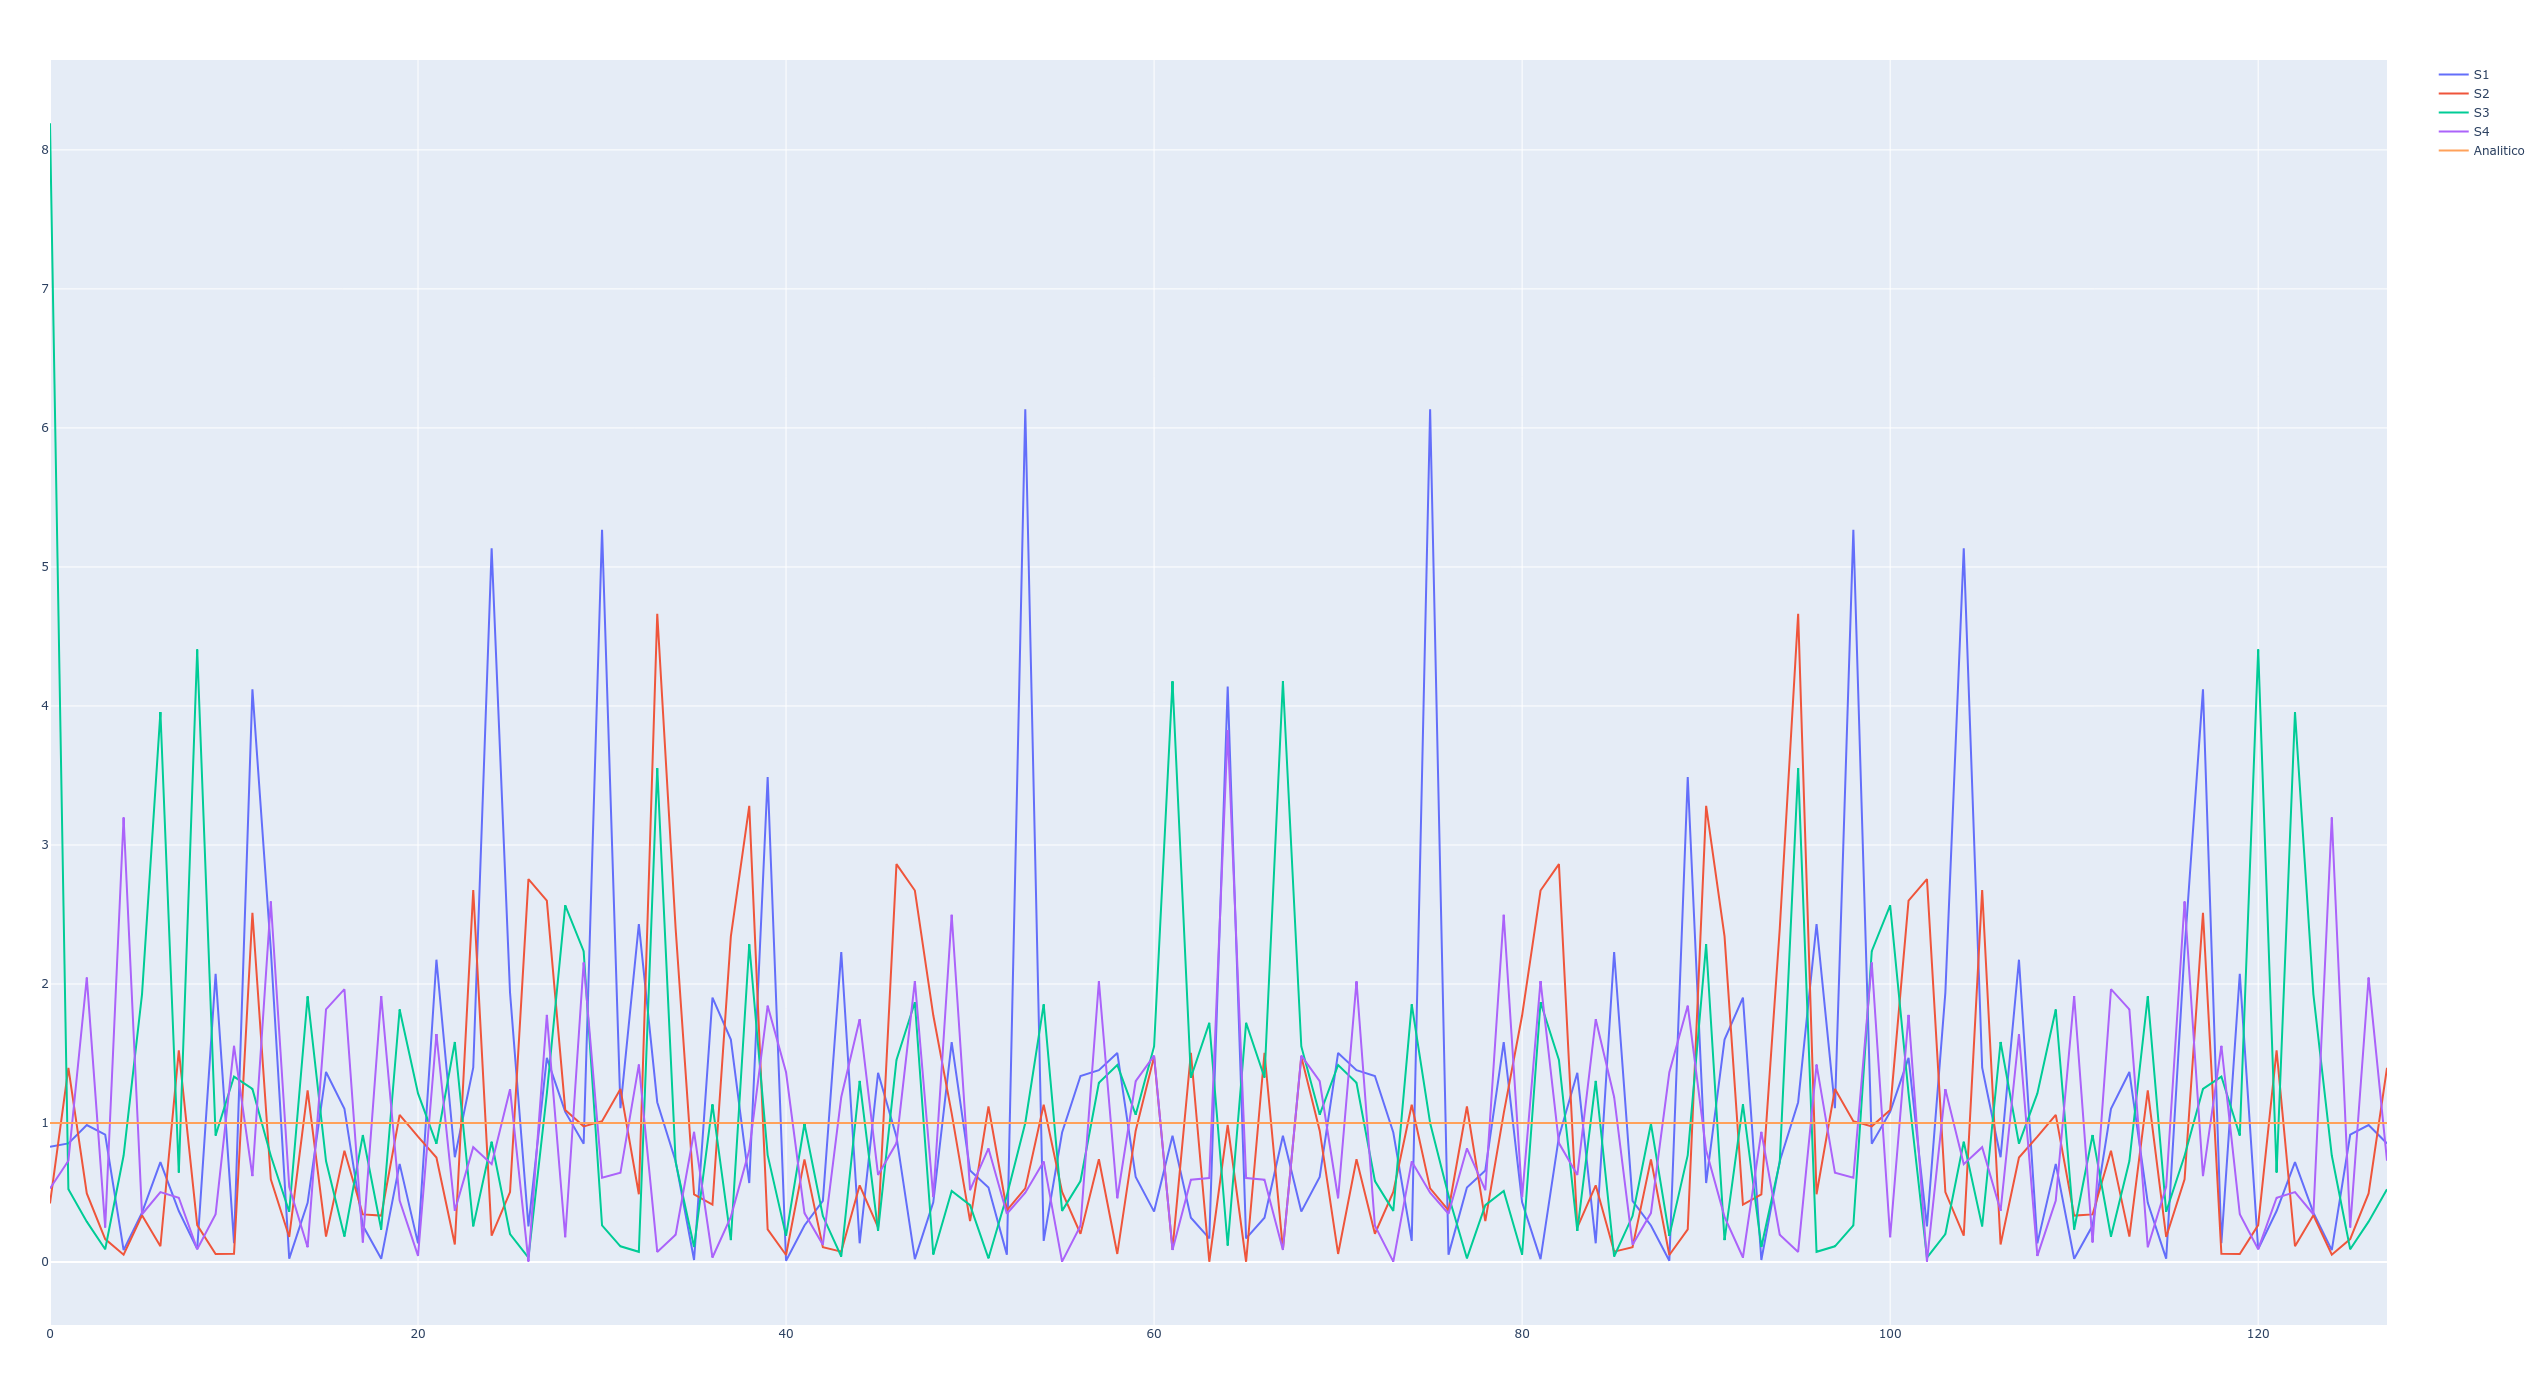
\includegraphics[width=18cm]{imagenes/4RealizacionesyAnalitico.png}
\caption{Periodograma de 4 realizaciones, junto al calculo analítico}
\end{figure}

\clearpage
\section{Ejercicio 3}

\begin{figure}[!ht]
\centering
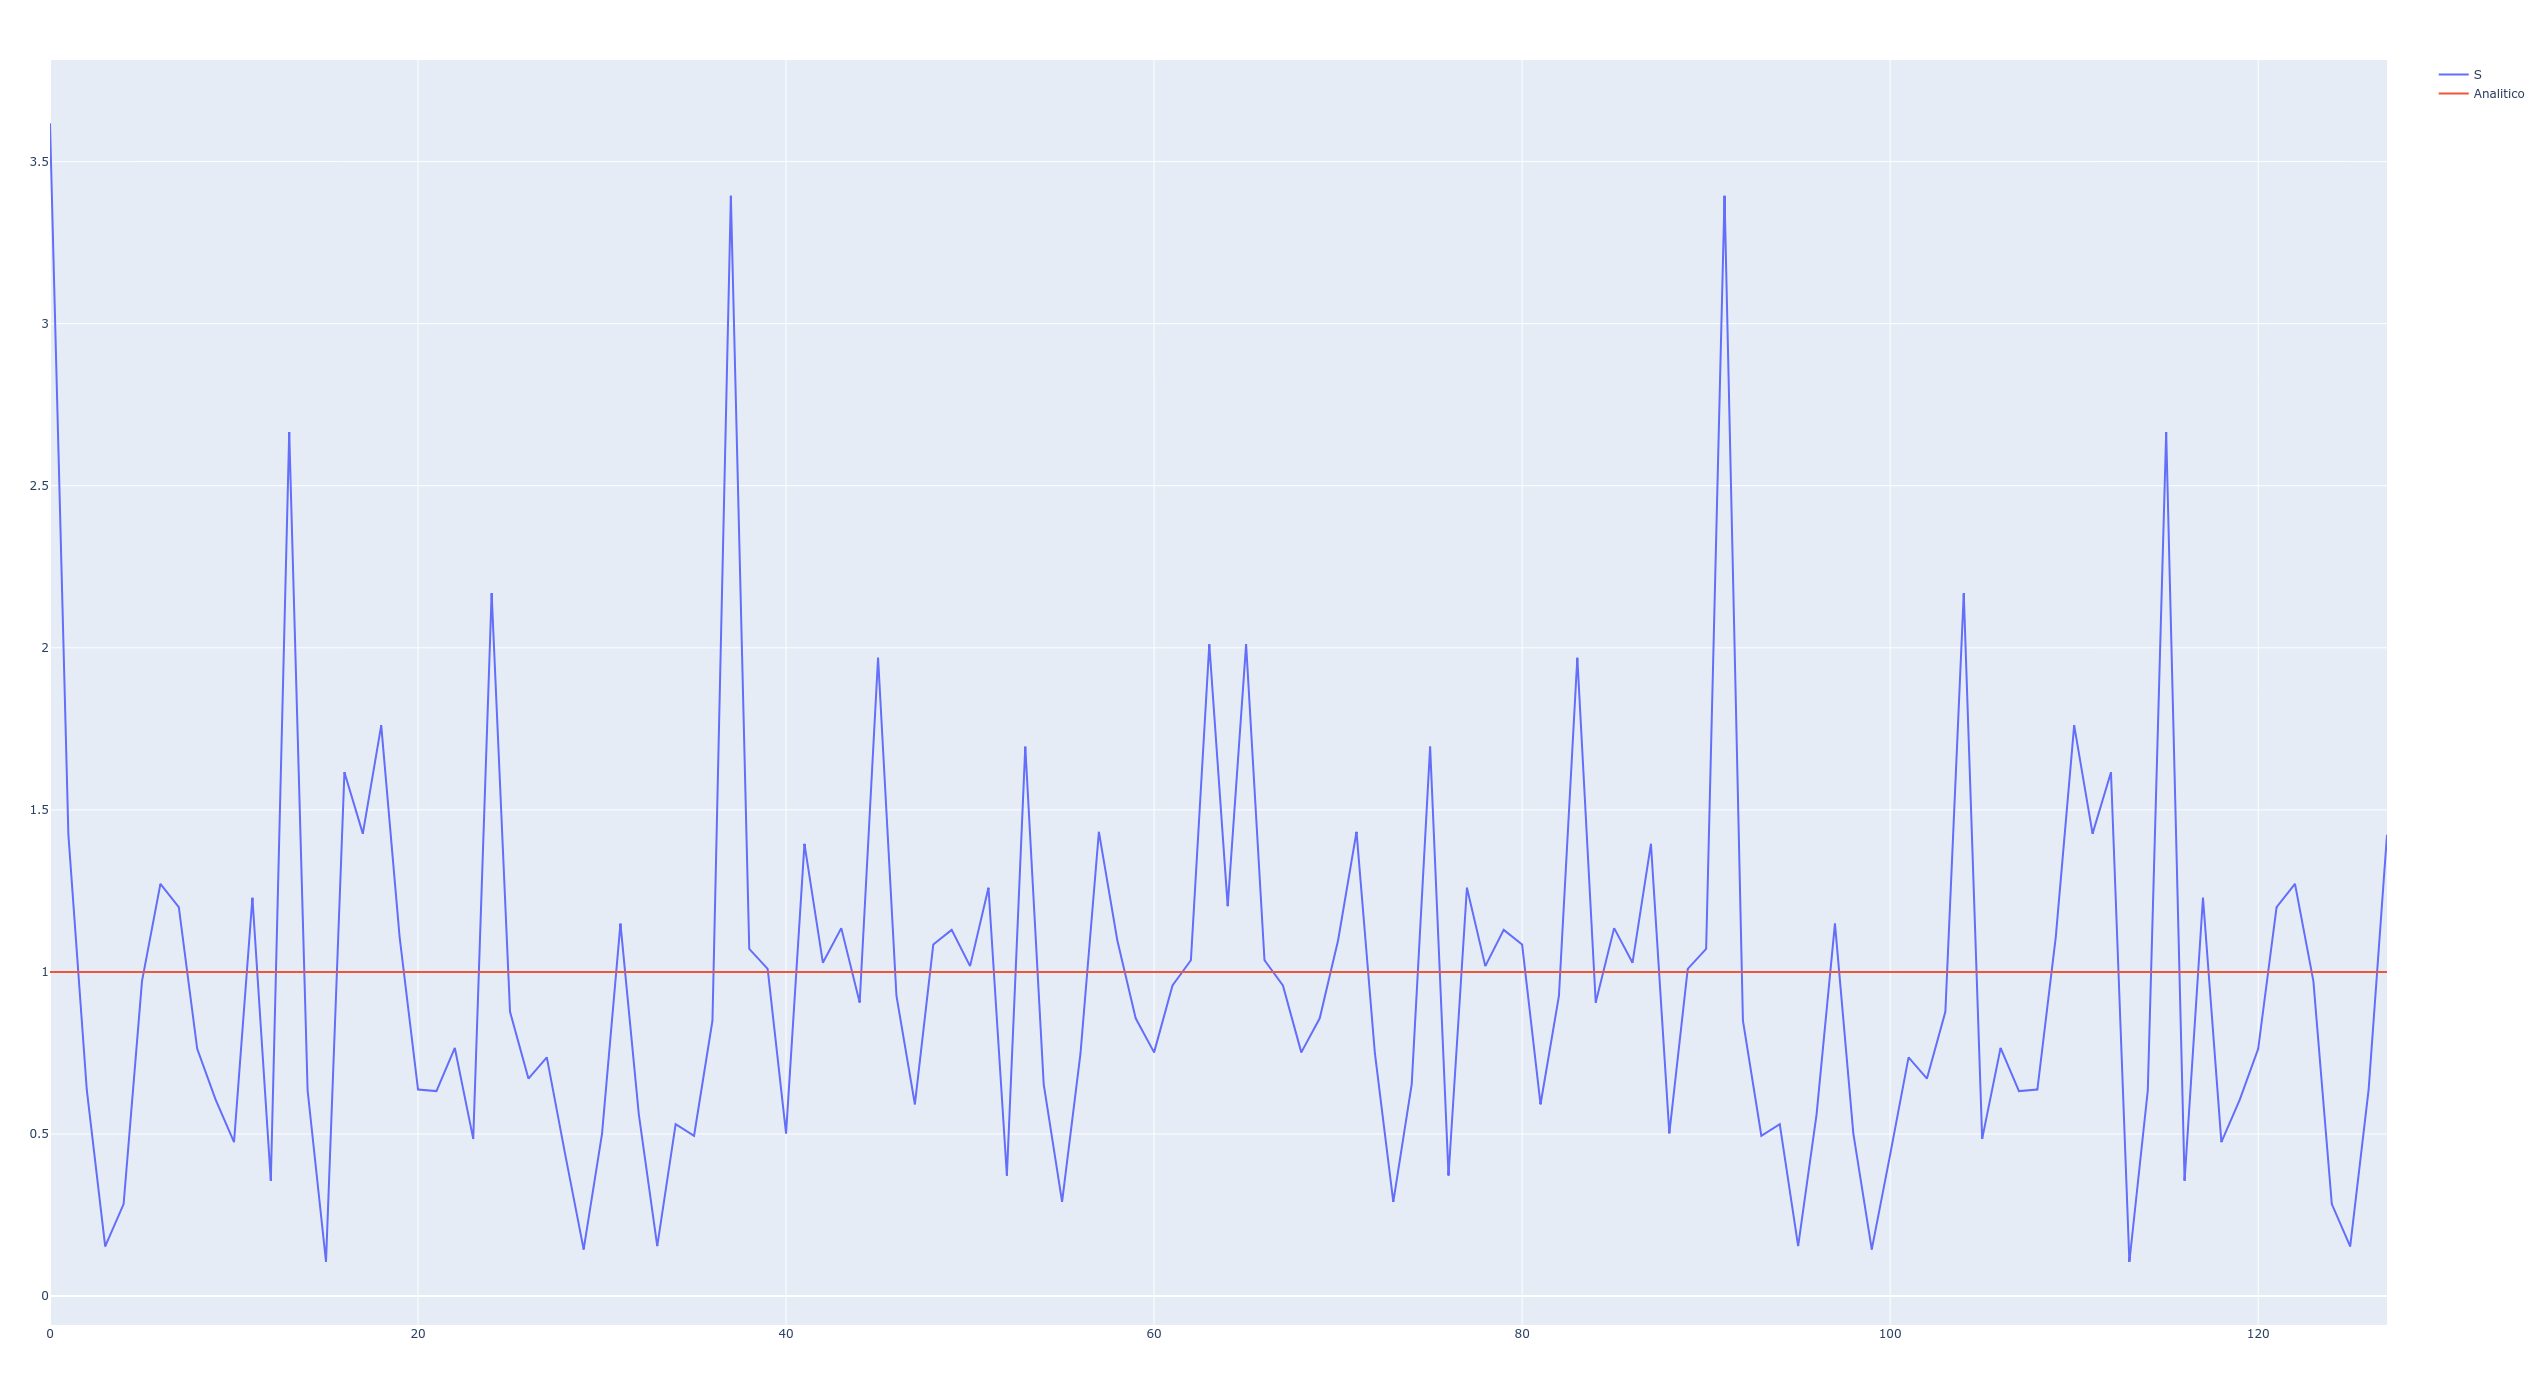
\includegraphics[width=18cm]{imagenes/PromedioN2.png}
\caption{Promedio de 2 periodogramas, junto al calculo analítico}
\end{figure}

\begin{figure}[!ht]
\centering
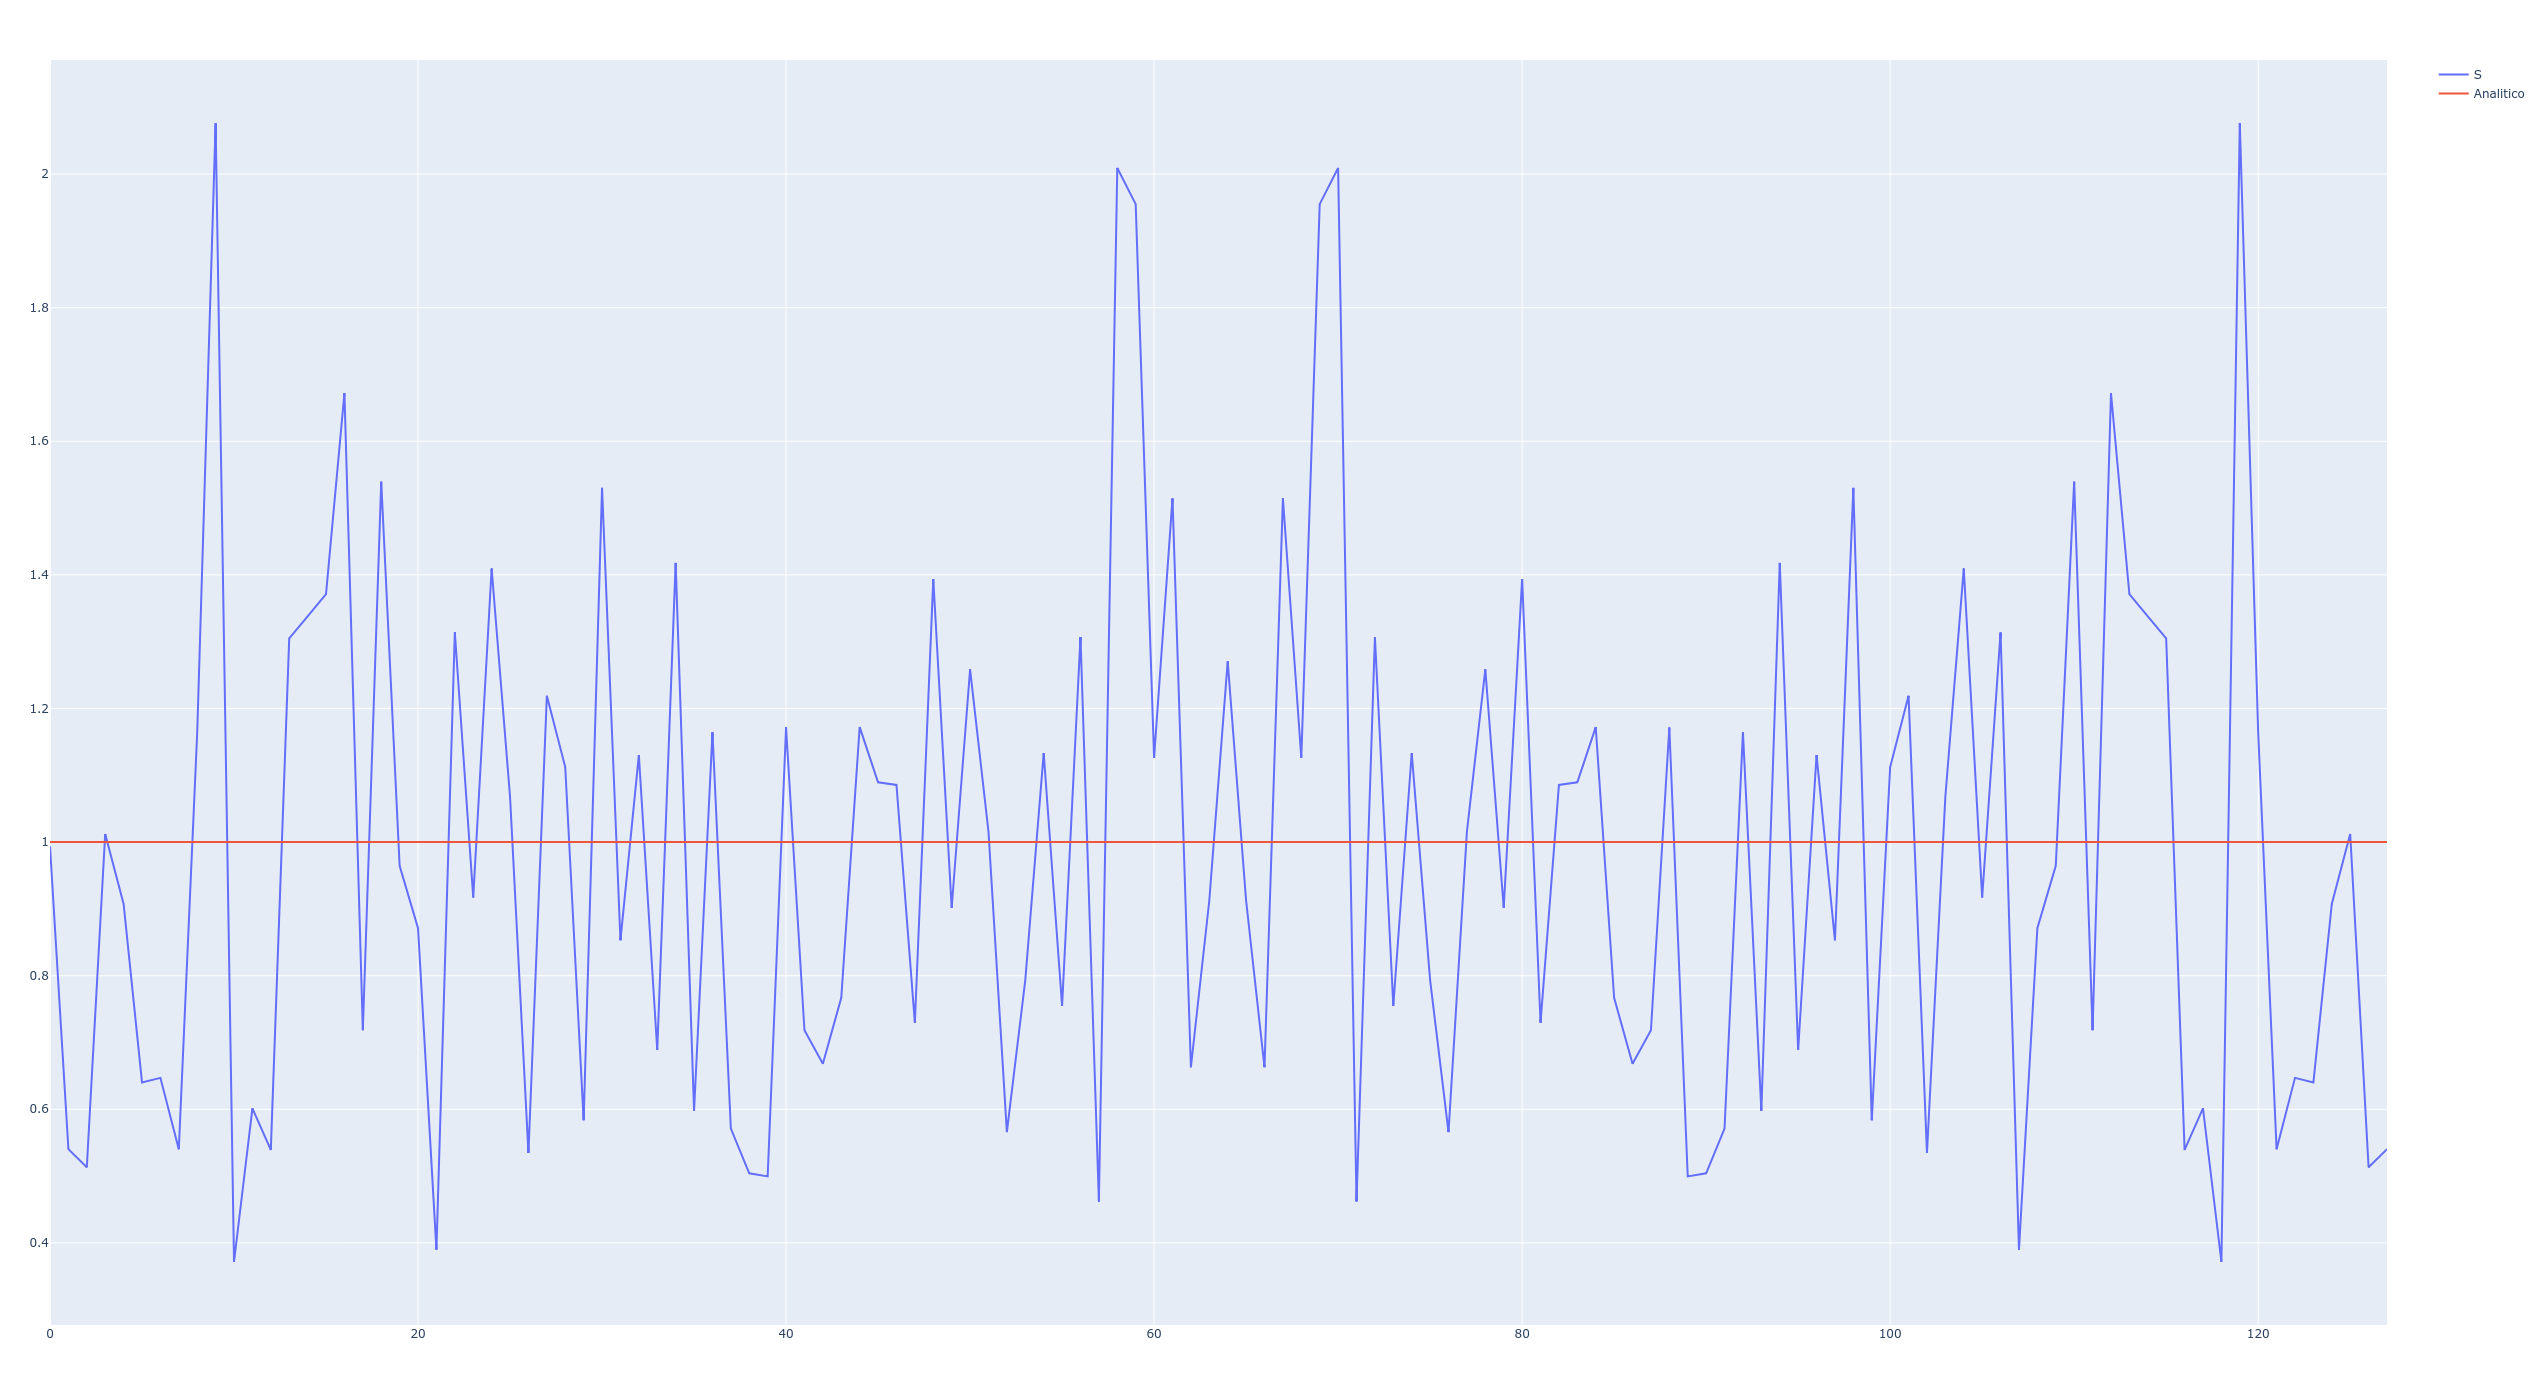
\includegraphics[width=18cm]{imagenes/PromedioN5.png}
\caption{Promedio de 5 periodogramas, junto al calculo analítico}
\end{figure}

\begin{figure}[!ht]
\centering
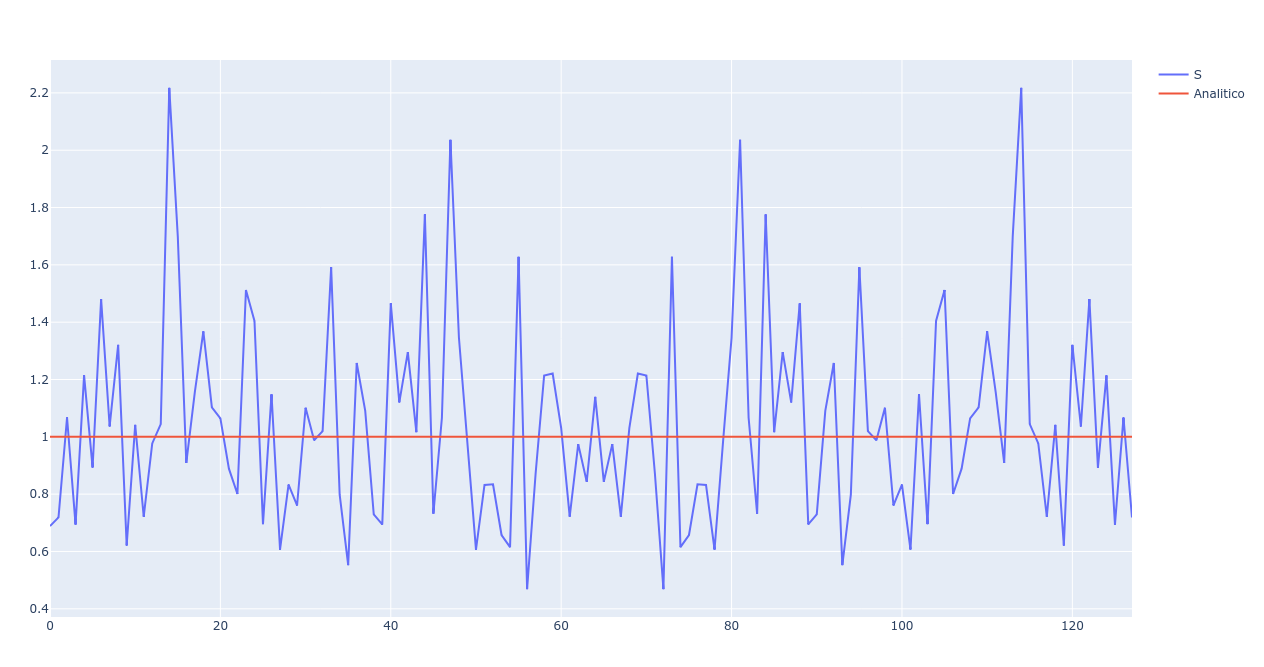
\includegraphics[width=18cm]{imagenes/PromedioN10.png}
\caption{Promedio de 10 periodogramas, junto al calculo analítico}
\end{figure}

\begin{figure}[!ht]
\centering
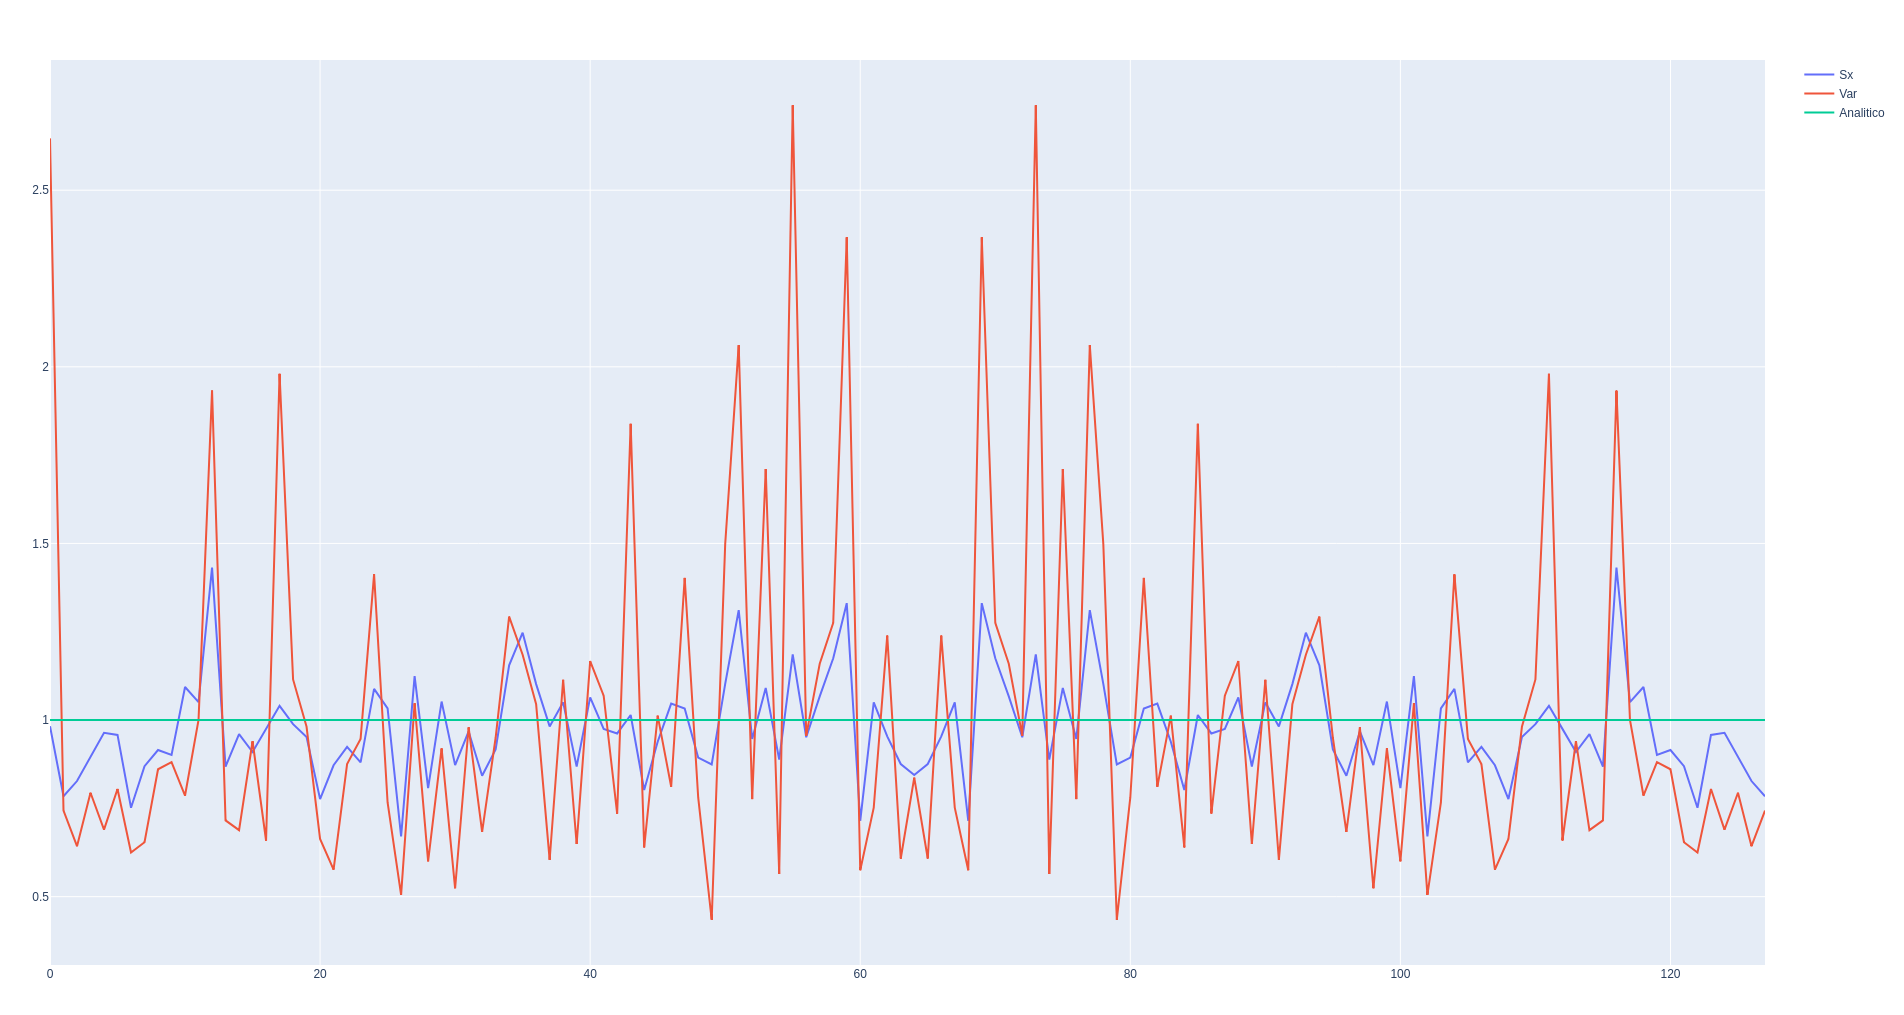
\includegraphics[width=18cm]{imagenes/PromedioN50.png}
\caption{Promedio de 50 periodogramas, junto al calculo analítico}
\end{figure}

\begin{figure}[!ht]
\centering
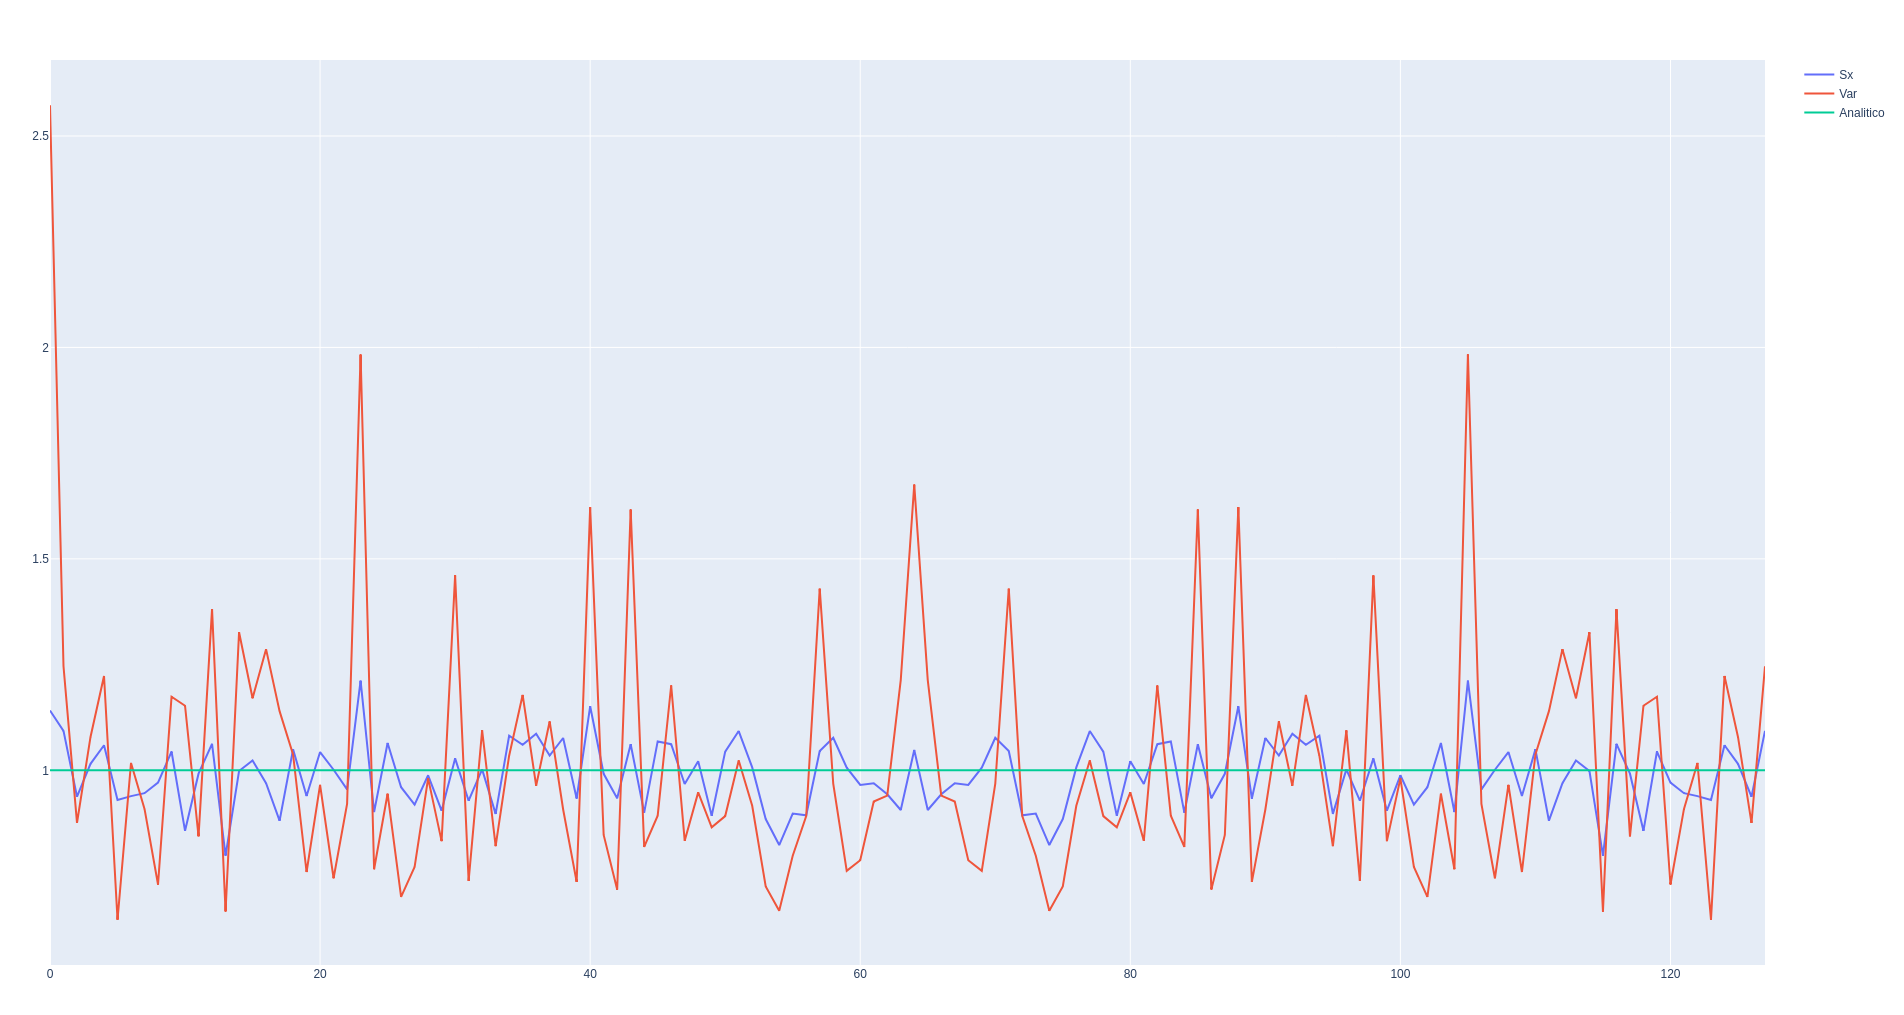
\includegraphics[width=18cm]{imagenes/PromedioN100.png}
\caption{Promedio de 100 periodogramas, junto al calculo analítico}
\end{figure}

\begin{figure}[!ht]
\centering
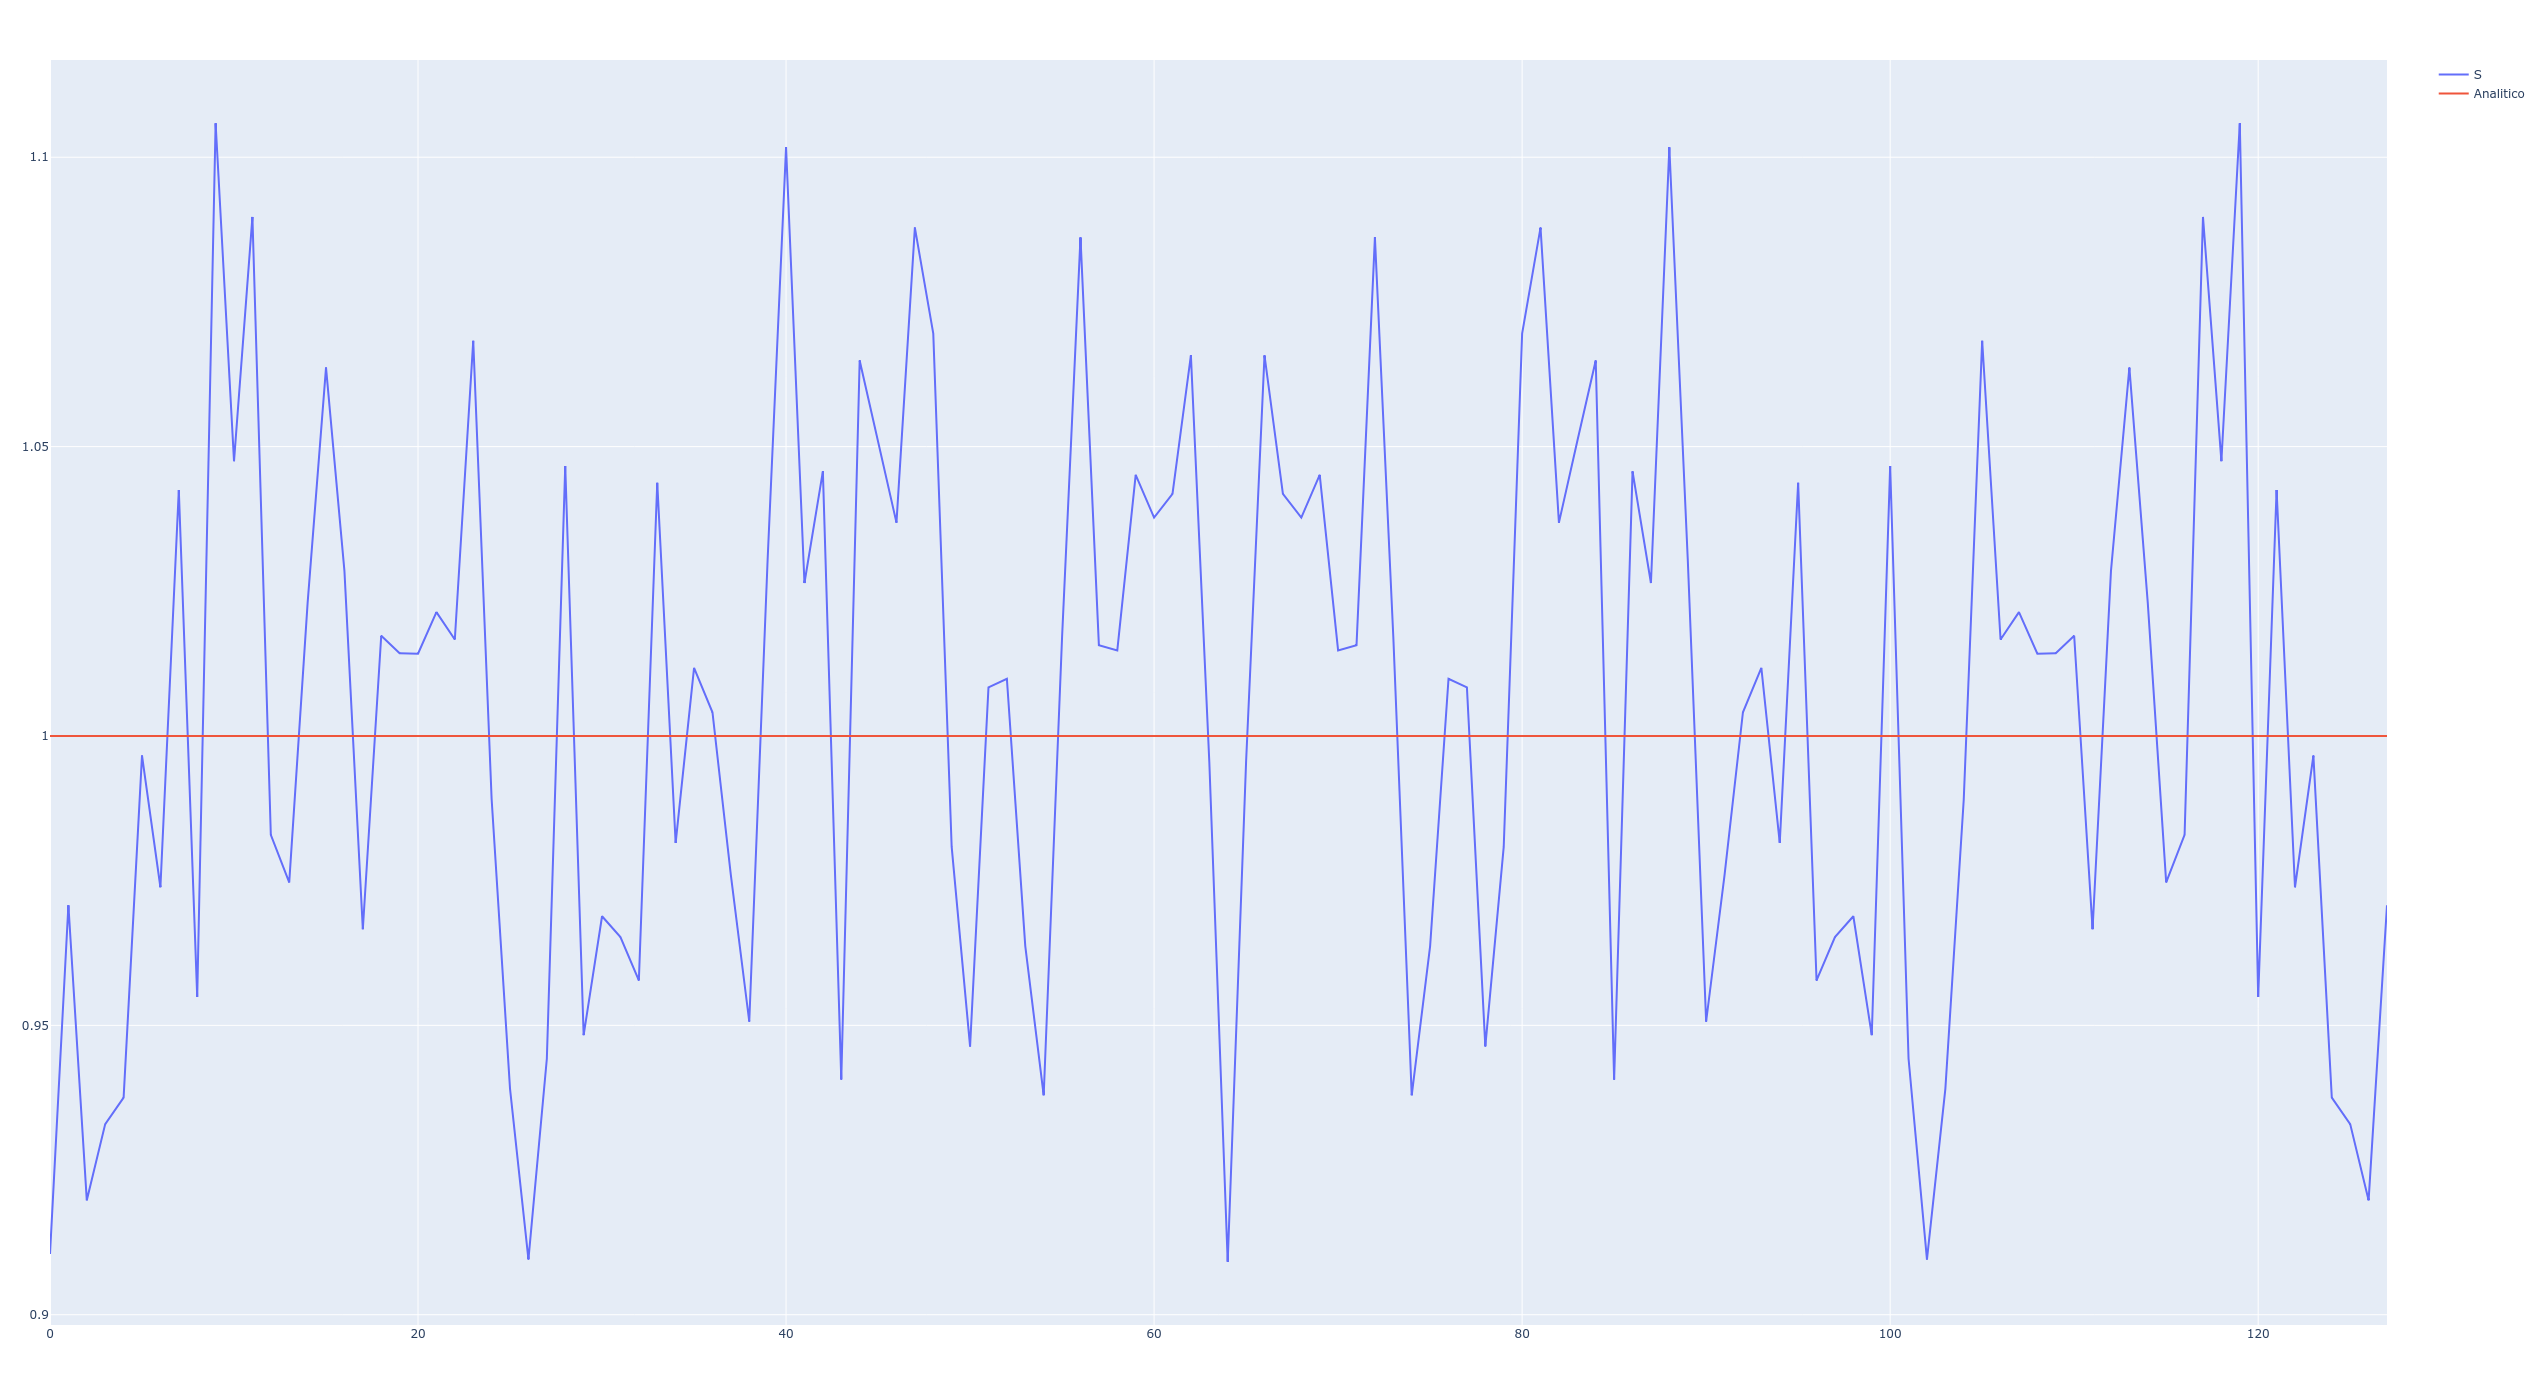
\includegraphics[width=18cm]{imagenes/PromedioN500.png}
\caption{Promedio de 500 periodogramas, junto al calculo analítico}
\end{figure}

\clearpage
\begin{equation*}
	\begin{split}
		Var \left[X_n(t)\right]=1\\
		\\
		Var\left[\frac{\sum_{n=0}^{N}X_n(t)}{N}\right]&=\frac{1}{N^2}\cdot Var\left[\sum_{n=0}^{N}X_n(t)\right]\\
		&=\frac{1}{N^{\cancel{2}}}\cdot \cancel{N}\cdot Var\left[X_n(t)\right]\\
		&=\frac{1}{N}\cdot Var\left[X_n(t)\right]\\
		Var\left[\frac{\sum_{n=0}^{N}X_n(t)}{N}\right]&=\frac{1}{N}
	\end{split}
\end{equation*}

\end{document}
